\documentclass{ximera}
%% You can put user macros here
%% However, you cannot make new environments

\listfiles

\graphicspath{{./}{firstExample/}{secondExample/}}

\usepackage{tikz}
\usepackage{tkz-euclide}
\usepackage{tikz-3dplot}
\usepackage{tikz-cd}
\usetikzlibrary{shapes.geometric}
\usetikzlibrary{arrows}
\usetkzobj{all}
\pgfplotsset{compat=1.13} % prevents compile error.

%\renewcommand{\vec}[1]{\mathbf{#1}}
\renewcommand{\vec}{\mathbf}
\newcommand{\RR}{\mathbb{R}}
\newcommand{\dfn}{\textit}
\newcommand{\dotp}{\cdot}
\newcommand{\id}{\text{id}}
\newcommand\norm[1]{\left\lVert#1\right\rVert}
 
\newtheorem{general}{Generalization}
\newtheorem{initprob}{Exploration Problem}

\tikzstyle geometryDiagrams=[ultra thick,color=blue!50!black]

%\DefineVerbatimEnvironment{octave}{Verbatim}{numbers=left,frame=lines,label=Octave,labelposition=topline}



\usepackage{mathtools}


\title{Where was Eye? Part I} \license{CC BY-NC-SA 4.0}

\begin{document}

\begin{abstract}
\end{abstract}
\maketitle

\section*{Where was Eye? Part I}

\begin{exploration}\label{exp:matchPic}
Three students, Adam, Benjamin, and Cayla, took part in a photography competition.  All three submitted photos of railroad tracks.  Adam and Benjamin took photos from their natural height; Cayla flew a drone high above her head to take a picture.
    \begin{image}
         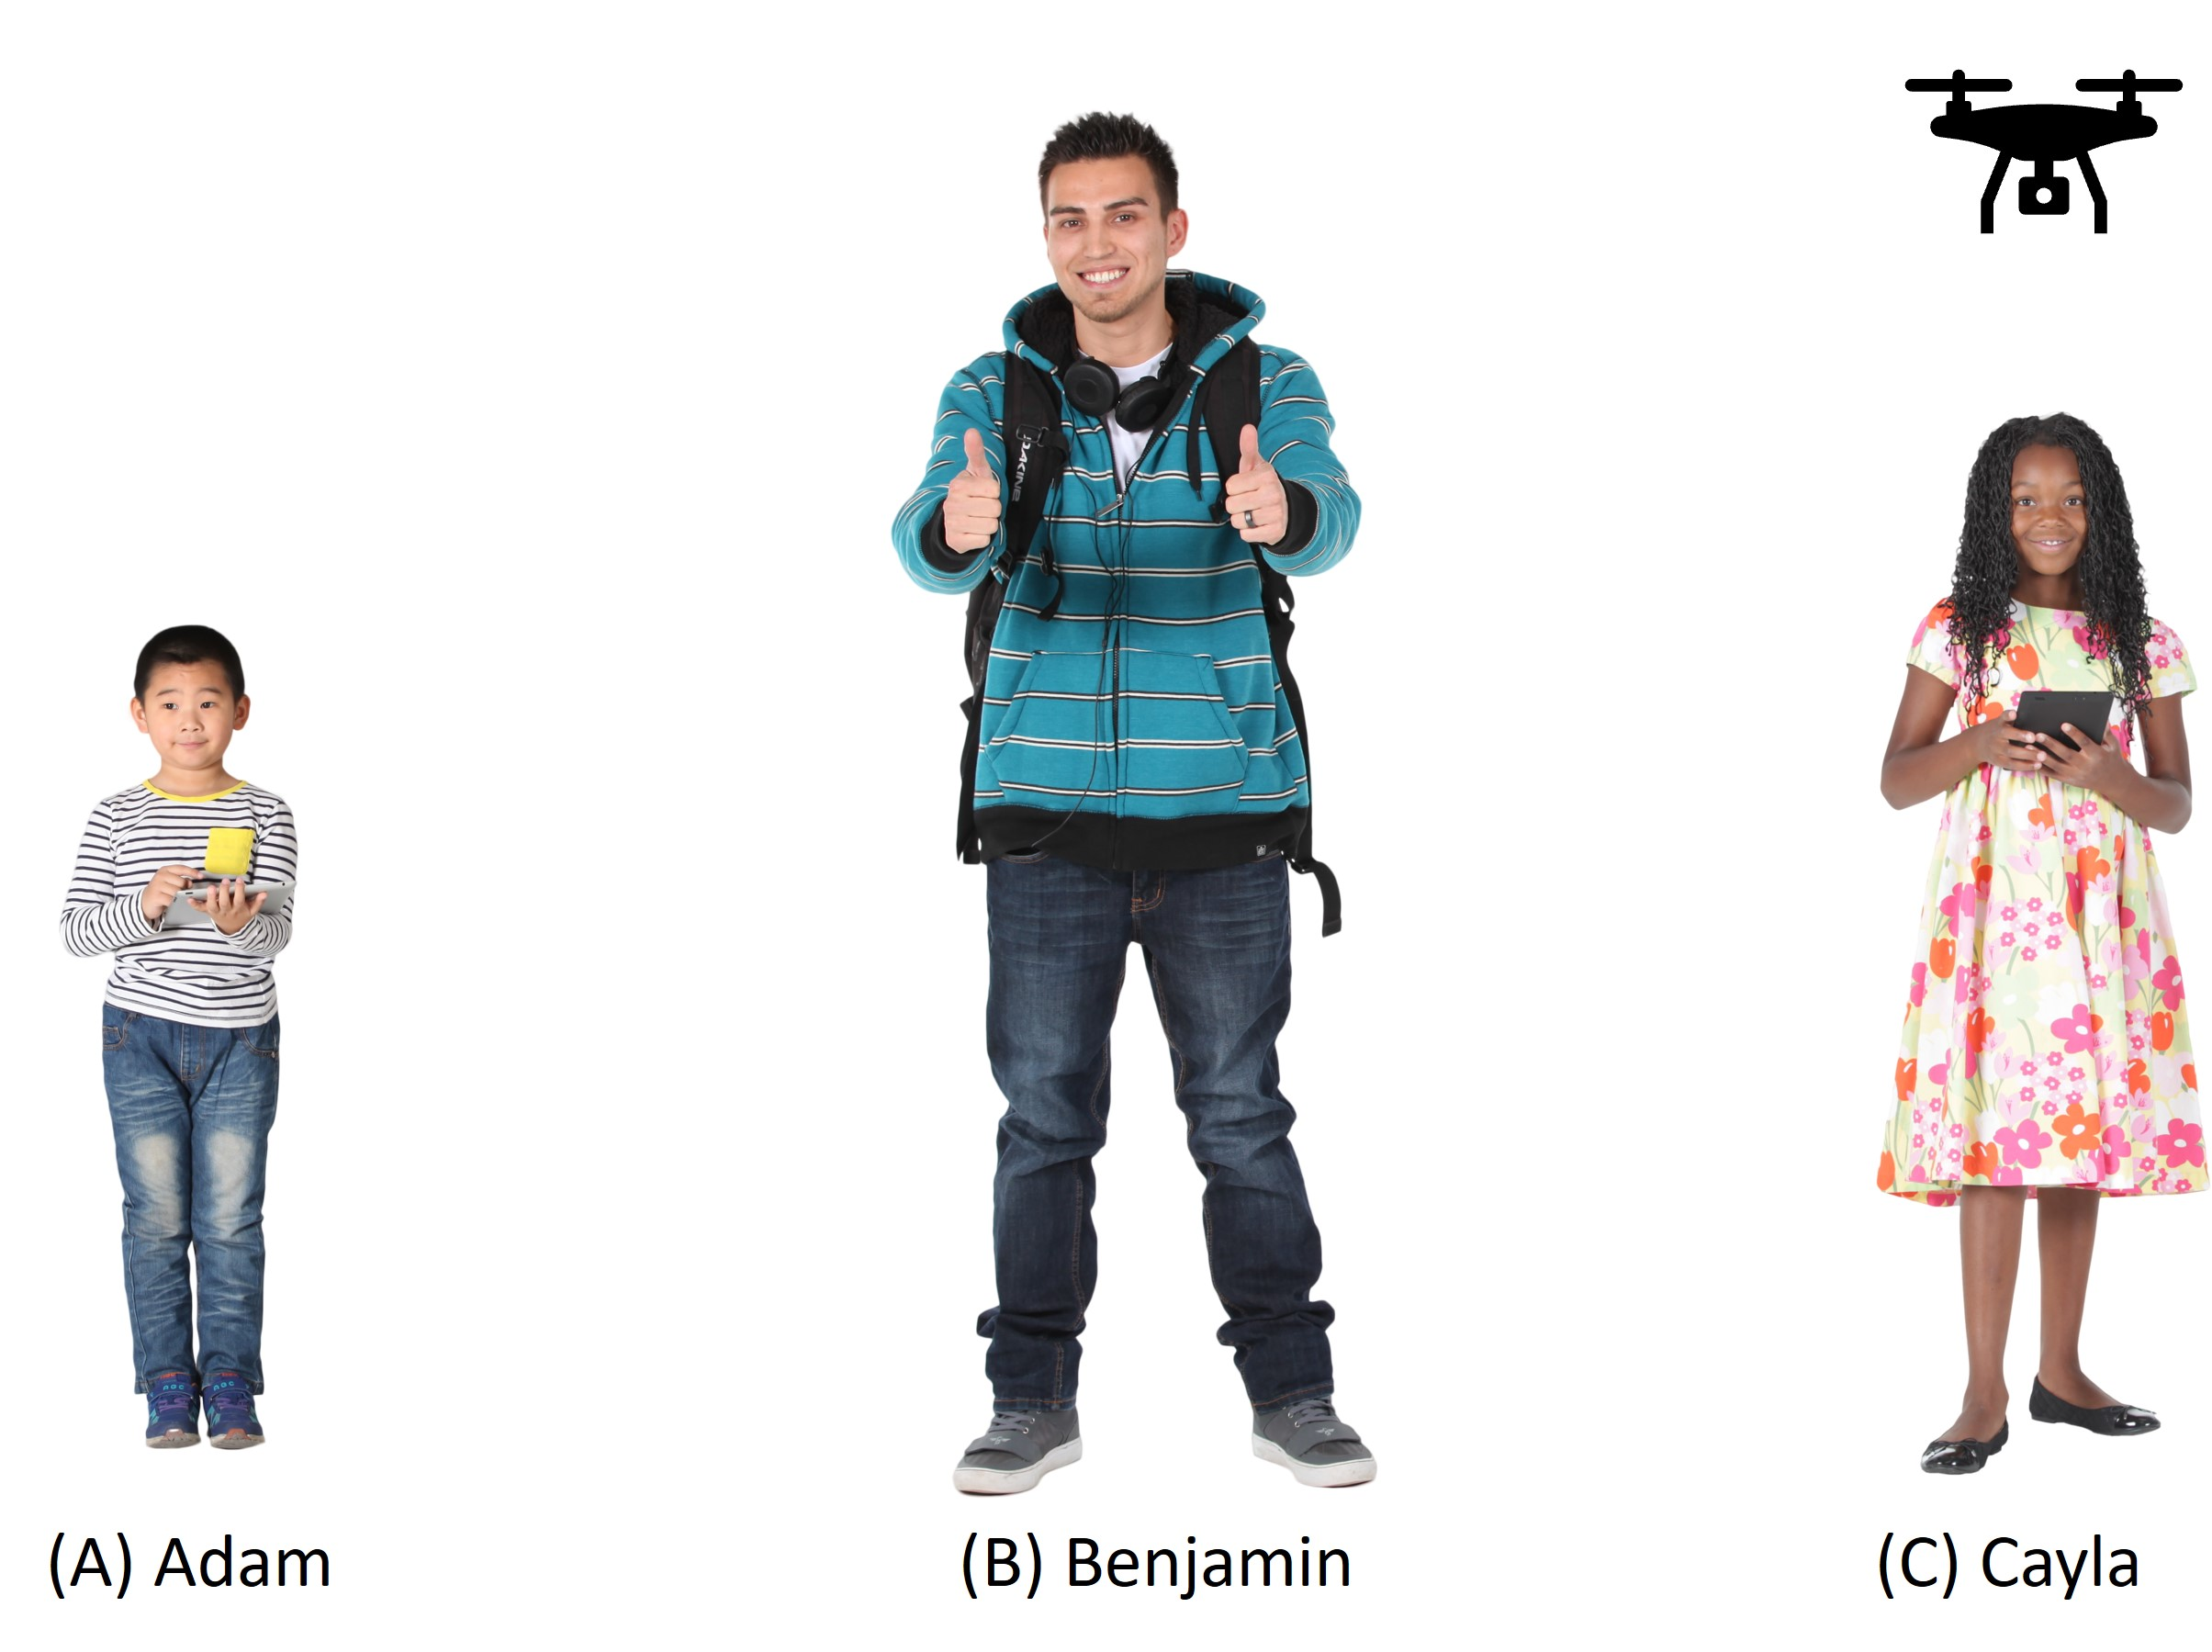
\includegraphics[width=4in]{AdamBenjaminCayla.jpg}
\end{image}
The images Adam, Benjamin, and Cayla took appear below (in no particular order).
\begin{image}
         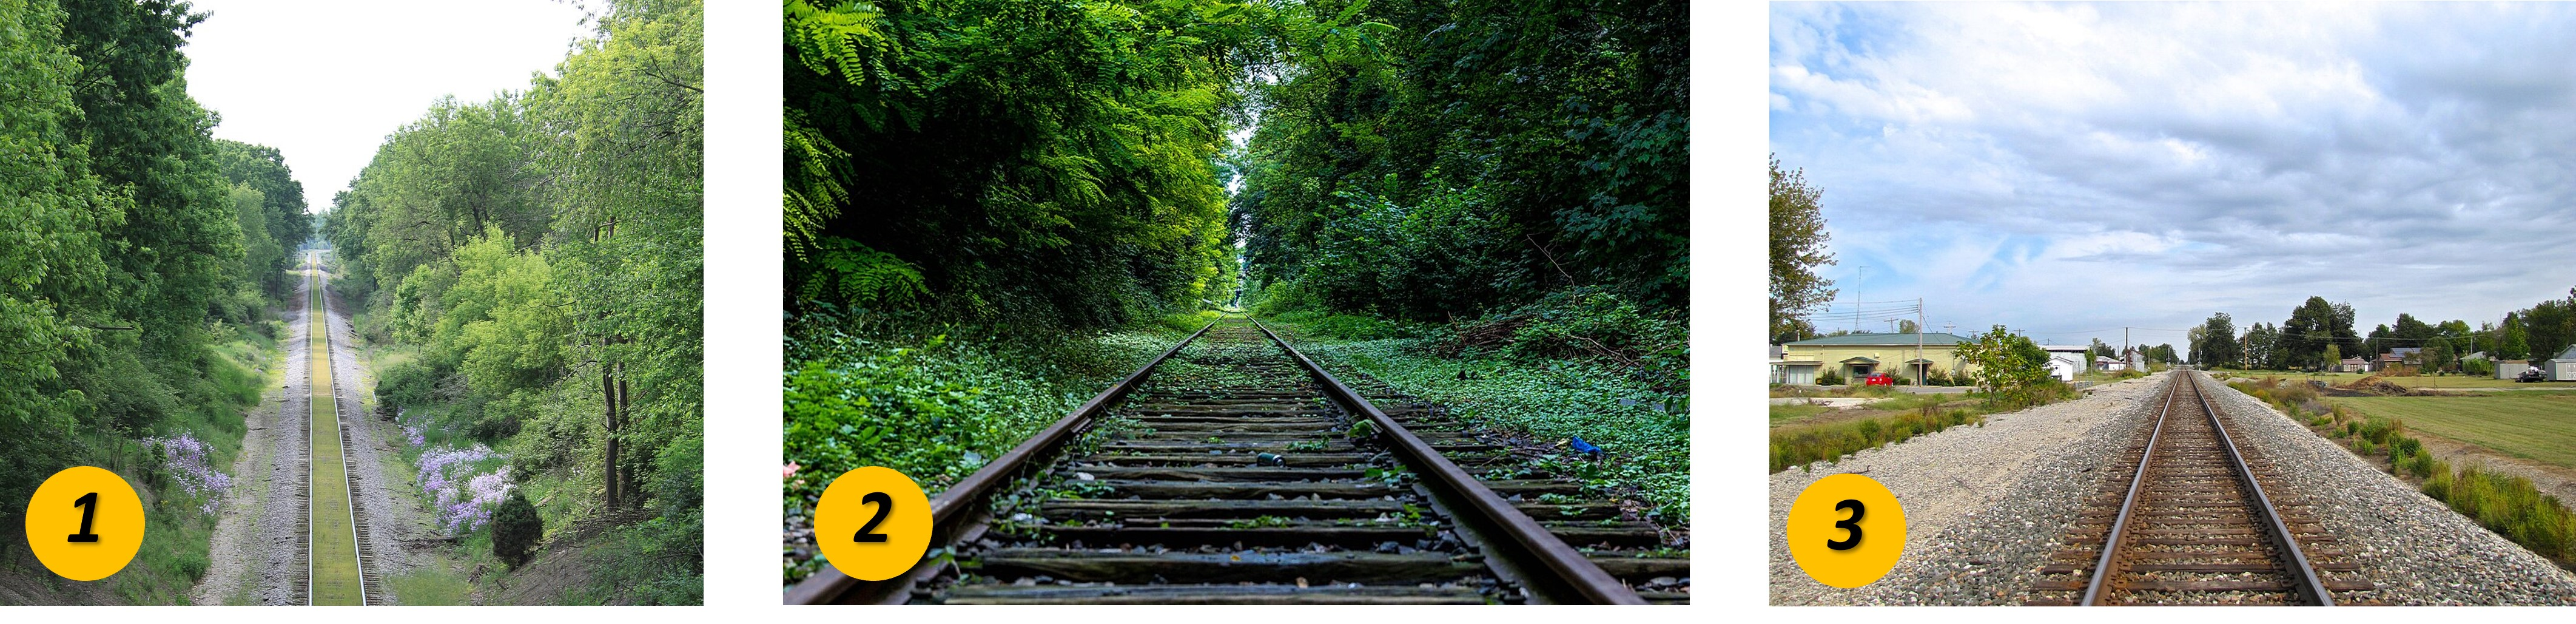
\includegraphics[width=5in]{threePics.jpg}
\end{image}
Match each image with the photographer who took it.

Photo 1 was taken by 
\begin{multipleChoice}
    \choice{Adam}
    \choice{Benjamin}
    \choice[correct]{Cayla}
\end{multipleChoice}

Photo 2 was taken by 
\begin{multipleChoice}
    \choice[correct]{Adam}
    \choice{Benjamin}
    \choice{Cayla}
\end{multipleChoice}

Photo 3 was taken by 
\begin{multipleChoice}
    \choice{Adam}
    \choice[correct]{Benjamin}
    \choice{Cayla}
\end{multipleChoice}

In small groups, discuss the reasons for your choices.  Do you think it is possible to use these photographs to estimate the height of the camera that took each photo?
\end{exploration}

\begin{exploration}\label{exp:trianglesAtBase}
    Let's look at the three pictures geometrically.  The rails appear to meet at a single point.  
    
\begin{image}
         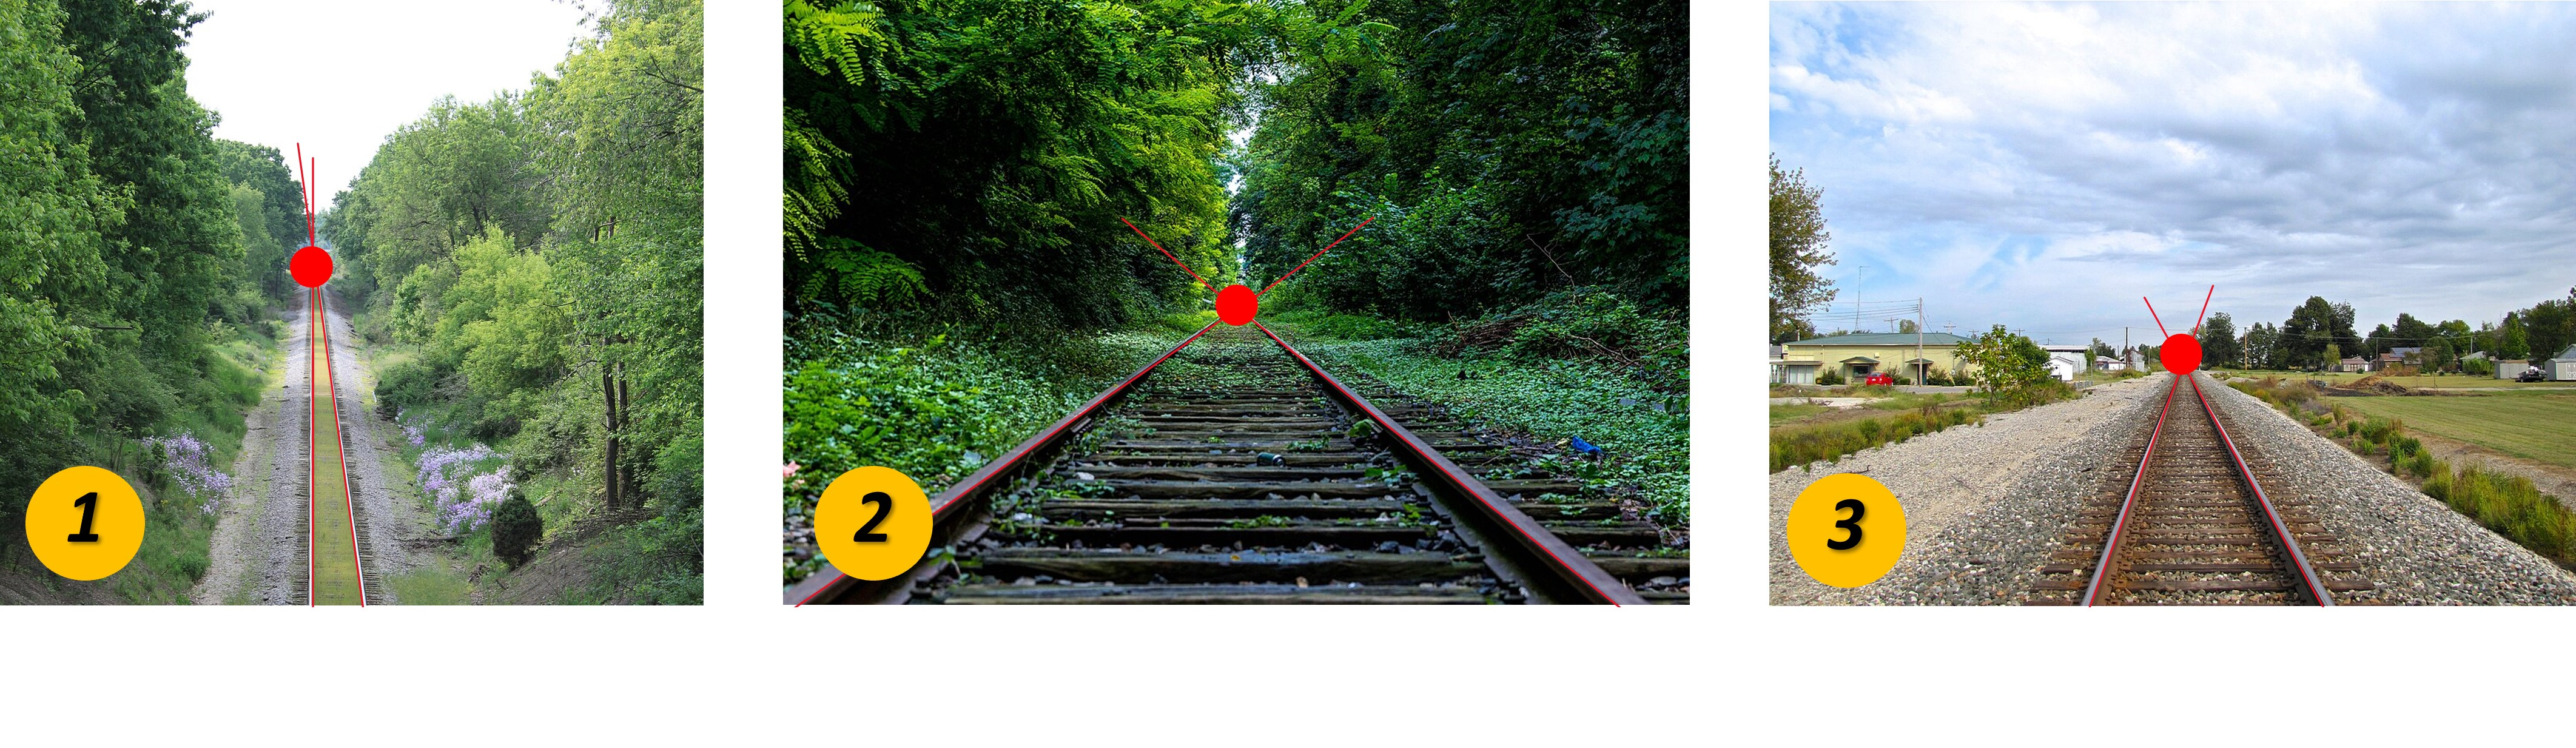
\includegraphics[width=5in]{vanishingPoint.jpg}
\end{image}
    
    Do you know what this point is called?
    \begin{multipleChoice}
        \choice{Center point}
        \choice[correct]{Vanishing point}
        \choice{Vertex}
        \choice{End point}
    \end{multipleChoice}

The rails, together with the bottom of each photo form triangles.  

\begin{image}
         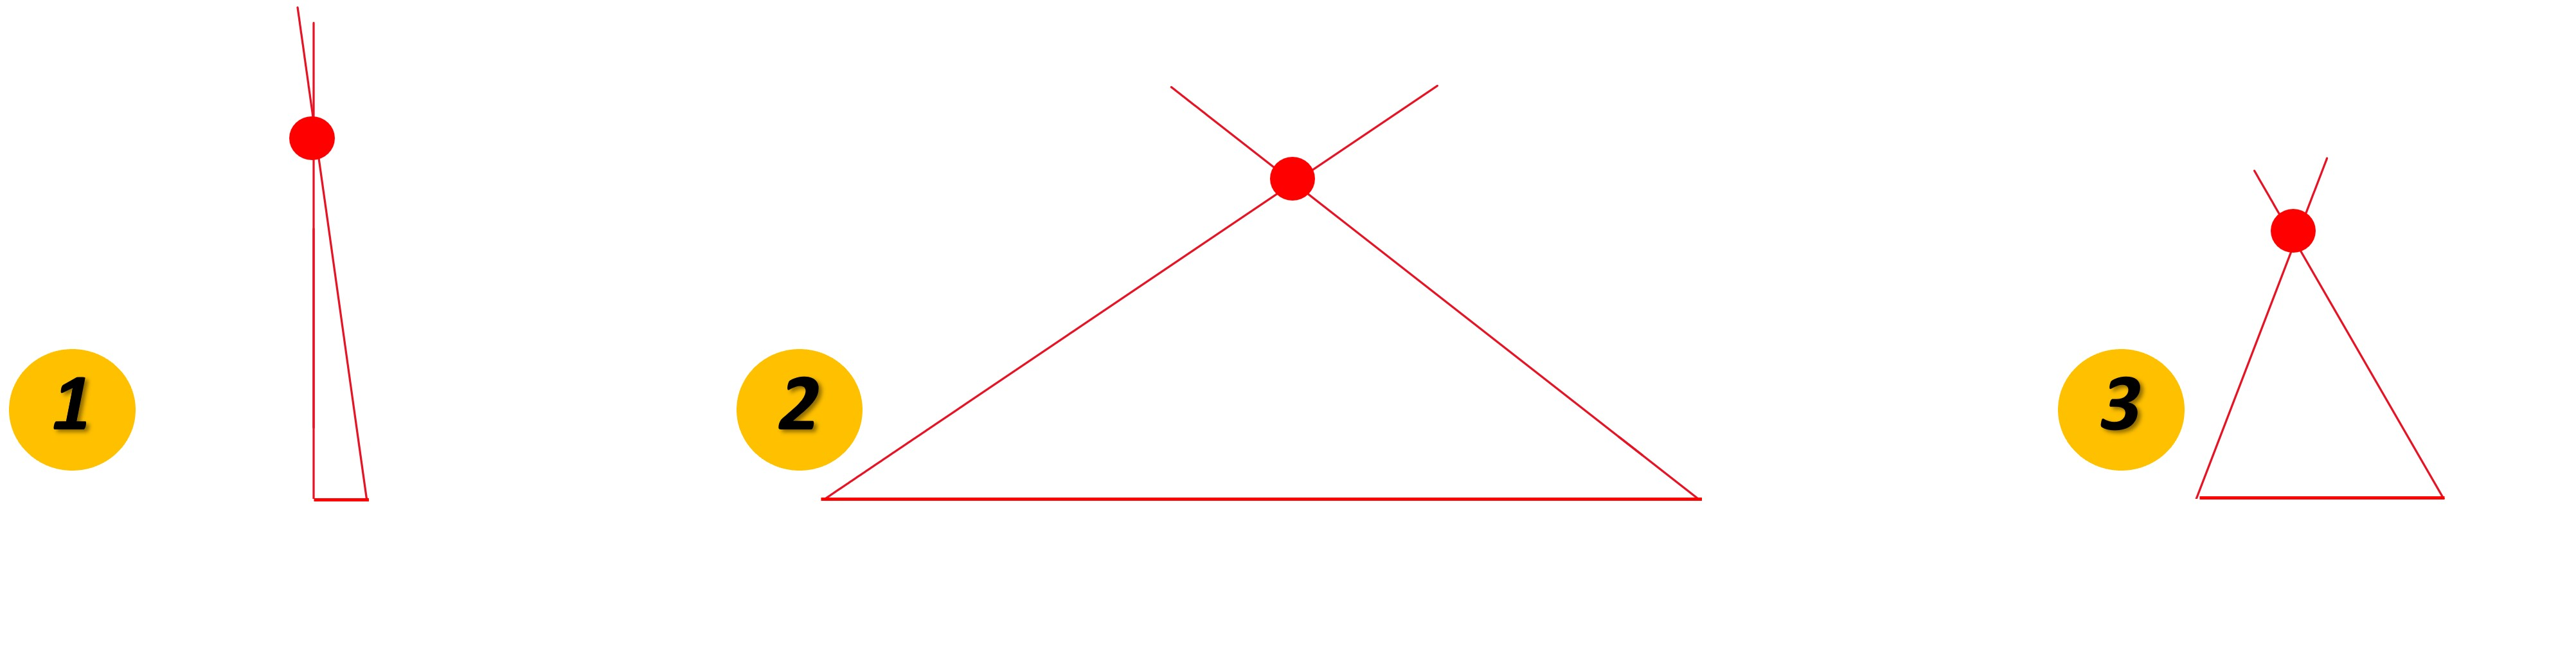
\includegraphics[width=5in]{triangles.jpg}
\end{image}

You might describe the first triangle as tall and narrow, and the second triangle as wide and short.  These descriptions refer to the \emph{proportions} of these triangles.  To really see the difference in the proportions, we can make the bases of the triangles the same size.  This makes sense to do because railroad tracks have the same width everywhere in the U.S.

\begin{image}
         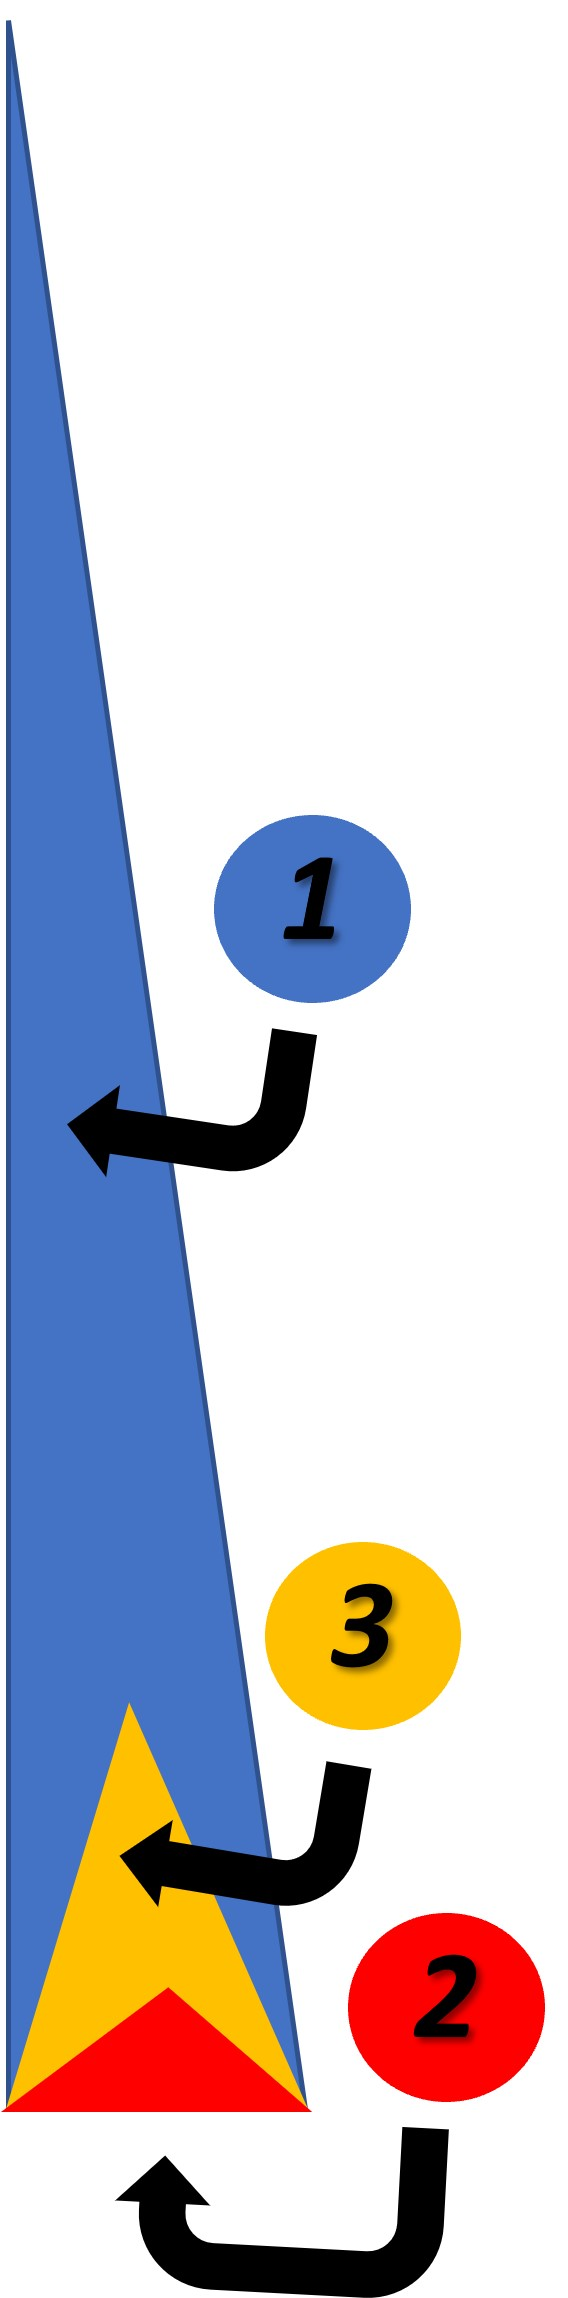
\includegraphics[width=3.5in]{matchedTriangles.jpg}
\end{image}



\end{exploration}

\end{document}